\documentclass{standalone}
\usepackage{tikz}
\begin{document}
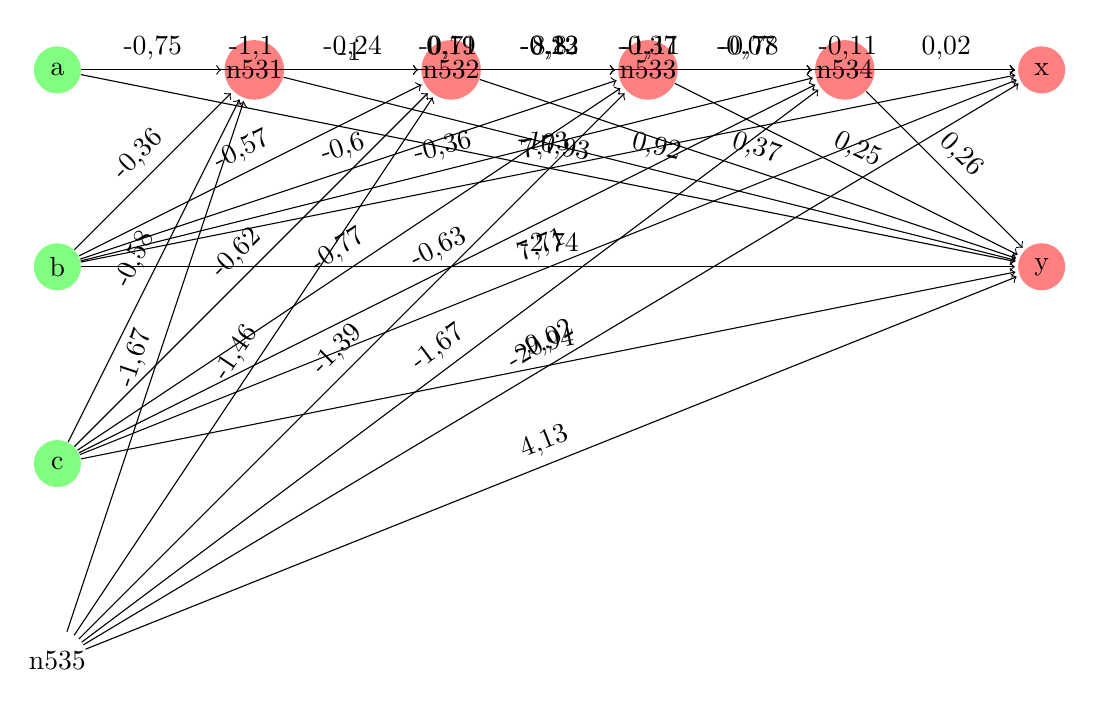
\begin{tikzpicture}[shorten >=1pt,->,draw=black!,node distance=2.5cm]
\tikzstyle{neuron}=[circle,fill=black!25,minimum size=17pt,inner sep=0pt]
\tikzstyle{constant}=[neuron, fill=white!50];
\tikzstyle{identity}=[neuron, fill=green!50];
\tikzstyle{sigmoid}=[neuron, fill=red!50];
\node [identity] (a) {a};
\node [identity,below of=a] (b) {b};
\node [identity,below of=b] (c) {c};
\node [constant,below of=c] (n535) {n535};
\node [sigmoid,right of=a] (n531) {n531};
\node [sigmoid,right of=n531] (n532) {n532};
\node [sigmoid,right of=n532] (n533) {n533};
\node [sigmoid,right of=n533] (n534) {n534};
\node [sigmoid,right of=n534] (x) {x};
\node [sigmoid,below of=x] (y) {y};
\path[every node/.style={sloped,anchor=south,auto=false}]
(b) edge node {-2,74} (y)
(b) edge node {7,73} (x)
(b) edge node {-0,57} (n532)
(b) edge node {-0,36} (n531)
(b) edge node {-0,36} (n534)
(b) edge node {-0,6} (n533)
(a) edge node {8,8} (x)
(a) edge node {-0,71} (n534)
(a) edge node {-0,75} (n531)
(a) edge node {-10,93} (y)
(a) edge node {-1} (n533)
(a) edge node {-1,1} (n532)
(c) edge node {7,71} (x)
(c) edge node {-0,58} (n531)
(c) edge node {-9,94} (y)
(c) edge node {-0,77} (n533)
(c) edge node {-0,62} (n532)
(c) edge node {-0,63} (n534)
(n532) edge node {0,37} (y)
(n532) edge node {-0,78} (x)
(n532) edge node {-0,37} (n534)
(n532) edge node {-0,22} (n533)
(n531) edge node {-1,11} (x)
(n531) edge node {0,92} (y)
(n531) edge node {0,19} (n533)
(n531) edge node {-0,24} (n532)
(n531) edge node {-0,13} (n534)
(n534) edge node {0,26} (y)
(n534) edge node {0,02} (x)
(n533) edge node {-0,11} (x)
(n533) edge node {0,25} (y)
(n533) edge node {-0,07} (n534)
(n535) edge node {-20,02} (x)
(n535) edge node {-1,67} (n531)
(n535) edge node {4,13} (y)
(n535) edge node {-1,39} (n533)
(n535) edge node {-1,46} (n532)
(n535) edge node {-1,67} (n534)
;\end{tikzpicture}
\end{document}